\section{Introduction}
\label{sec:intro}

Recent measurements of the inclusive forward-backward $t\bar{t}$ production asymmetry from the 
Tevatron experiments show deviations from the standard model (SM) expectations~\cite{d0:fwtop, cdf:fwtop1, cdf:fwtop2}.
The largest (3$\sigma$) deviation~\cite{cdf:fwtop2} is found to be in the region of high invariant mass with $M_{t\bar{t}} >  450$ GeV. 
Several attempts have been made to explain this asymmetry~\cite{berger, Buckley, Gresham, zoltan}. 
One of the natural modes where such an asymmetry could be induced is via the appearance of Flavor Changing Neutral Currents (FCNC) in the quark sector. 
Several extenstions of the SM can generate these couplings at tree level~\cite{hills, others1}.

At the LHC, FCNC processes such as $uu \rightarrow tt$ can be produced via the exchange of a $Z'$ boson, 
and can appear naturally in Techicolor (TC2) models or in general theories with non-universal massive neutral vector bosons. 
In these models the heavy boson couples strongly to the third generation of quarks, inducing FCNC. 
An enhancement of same-sign top pair production at the LHC via the exchange of a $Z'$ boson is predicted
by a very recent study of the forward-backward asymmetry ~\cite{berger}.
This detailed study also provides an explanation of the observed asymmetry at the Tevatron. 

This approach requires an interaction of $u-t-Z'$ with:

\begin{equation}
  \mathcal{L} = g_W \bar{u} \gamma^\mu (f_L P_L + f_R P_R)tZ'_\mu + h.c
\end{equation}

where $g_W$ is the weak coupling strength. The left-handed coupling is set to $f_L = 0$, due 
to the $B_d-\bar{B_d}$ mixing constraint~\cite{Cao}. The right-handed coupling $f_R$ is chosen to be a free parameter. 
Fig.~\ref{fig:tchannel} shows the t-channel exchange diagrams that can lead to the same-sign $tt$ final state. 
The initial state involves two $u-$quarks and thus the cross section at the LHC is enhanced due to the large valance quark parton density of the proton. 
As expected the coupling appears twice in the Feynman diagrams, thus the predicated rate is proportional to $f_R^4$. 

\begin{figure}[htb]
\begin{center}
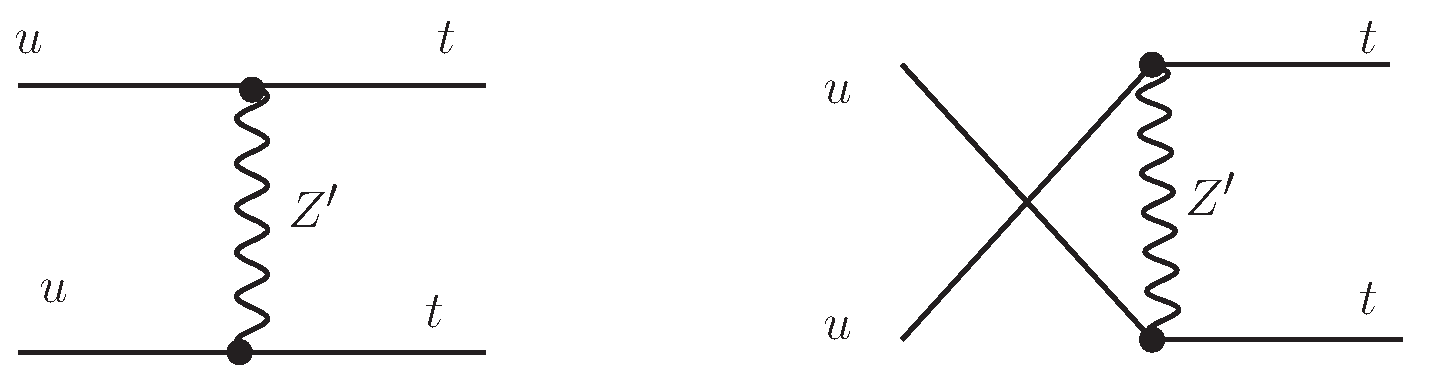
\includegraphics[width=0.7\linewidth, height=0.2\linewidth]{figs/sstop1.pdf}
\caption{ Diagrams for $tt$ pair production induced by $Z'$ exchange in t-channel. \label{fig:tchannel}}
\end{center}
\end{figure}

The s-channel production mode, in which the same-sign $tt$ pair is produced in association with a jet is shown in Fig.~\ref{fig:schannel}. 
The invarient mass of the $Z'$ can be recontructed using top quarks decay modes with an additional jet in the final state. 
As one of the initial parton is gluon initiated, we expect this rate to be lower than the t-channel diagram. 

\begin{figure}[htb]
\begin{center}
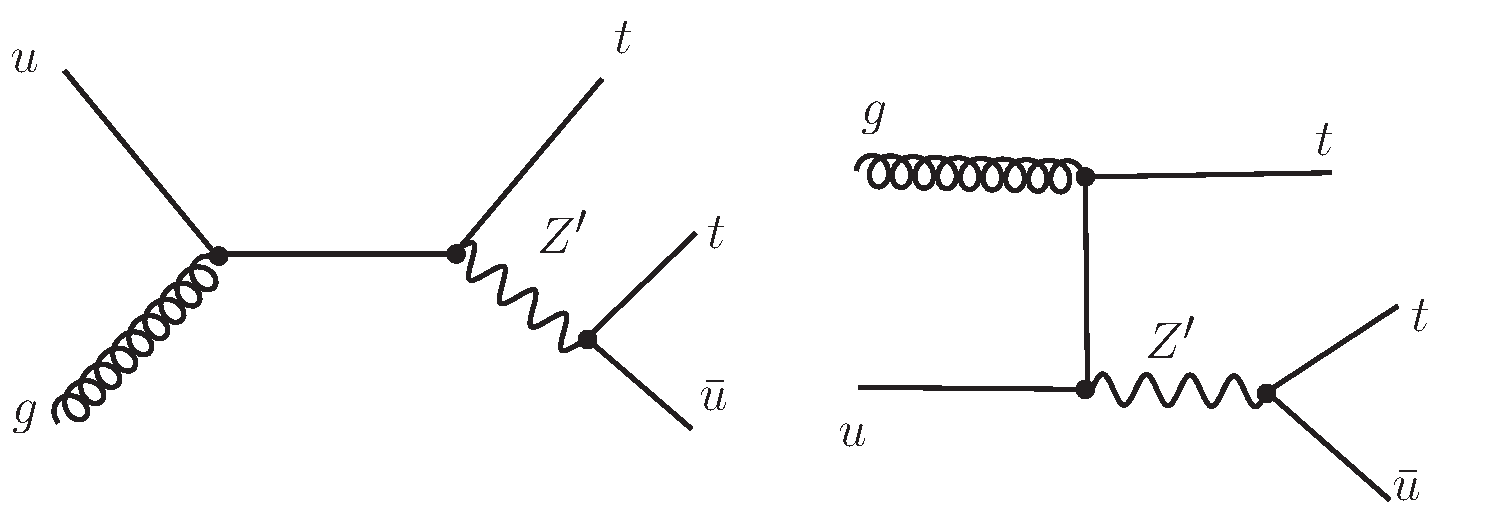
\includegraphics[width=0.7\linewidth, height=0.25\linewidth]{figs/sstop2.pdf}
\caption{ Diagrams for $tt\bar{u}$ production induced by $Z'$ exchange. \label{fig:schannel}}
\end{center}
\end{figure}

We use $\alpha_Sf_R^2$ as the proportionality constant for the production cross section. 
The width of the $Z'$ boson in this case is computed using BRIDGE~\cite{bridge} and verified using MadGraph~\cite{madgraph}. 
The total production cross sections for $tt$ and $ttj$ at the leading-order (LO) are shown as a function of $Z'$ mass in Fig.~\ref{fig:sstopcross}. 
The signal events are generated using the external model interface in MadGraph/MadEvent~\cite{madgraph}, 
with CTEQ6L~\cite{cteq6l} parton distribution function (PDF). The renormalization and factorization scales are chosen to be at the top mass scale ($m_{t} = 172.5$ GeV). 
The cross sections agree well with the published literature~\cite{berger}. 

\begin{figure}[htb]
\begin{center}
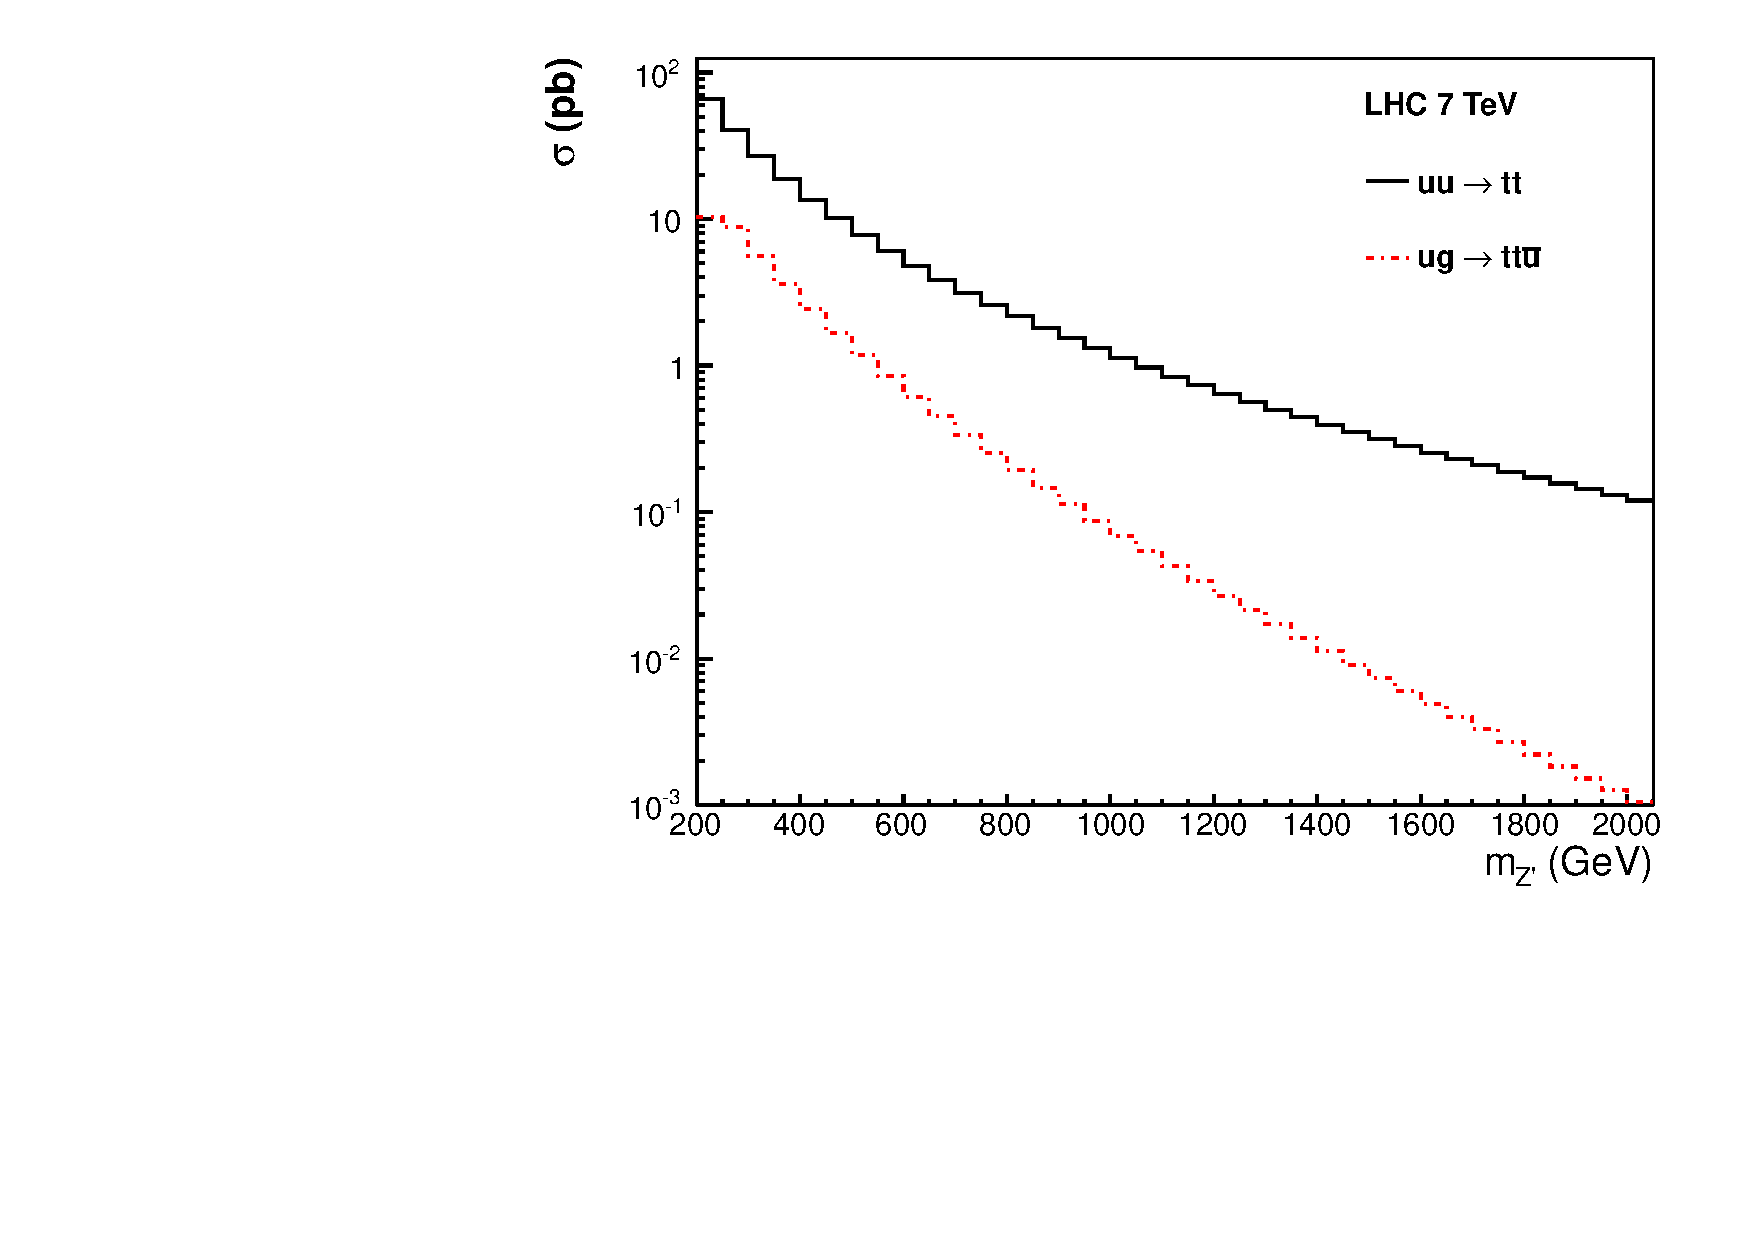
\includegraphics[width=0.7\linewidth]{figs/sstopcross.pdf}
\caption{ LHC production cross section for $tt$ and $ttj$ diagrams using right-handed coupling, $f_R = 1$. 
The renormalization and factorization scales are set to the top mass. \label{fig:sstopcross}}
\end{center}
\end{figure}

In this study we search for same-sign di-leptons originating from $tt$ or $ttj$ pair production as described above.
%in the $W^+ b W^+ b$ final states, where $W^+ \rightarrow l^+ \nu$. 
To do this we exploit the approved CMS results on same sign di-leptons documented in~\cite{ssnote1, sspaper}.
This note is organized as follows: 
in Section~\ref{sec:samesign} we give an overview of the method and results of Reference \cite{sspaper}
and we explain how these can be re-interpreted to set a limit on same-sign top production.
In Section~\ref{sec:ssresults} we present the the exclusion limit derived as a function of the mass and coupling of the $Z'$ boson.
Finally, in Section~\ref{sec:conclusion} we summarize the results.  


%The note is organized as follows: in Section~\ref{sec:datasamples} we list the data samples used in this analysis; 
%in Section~\ref{sec:eventselection} we describe the same sign di-lepton event selection; in Section~\ref{sec:samesign} 
%we discuss the results followed by the exclusion limits in Section~\ref{sec:ssresults}. Finally, in Section~\ref{sec:conclusion} 
%we summarize the results.  
%
%The work presented here is based on previously documented studies in~\cite{ssnote1, sspaper}.
